\documentclass[10pt,a4paper]{article}
\usepackage[margin=23mm]{geometry}
\usepackage[T1]{fontenc}
\usepackage{lmodern,microtype,amsmath,amssymb,amsthm,mathtools}
\usepackage{booktabs,longtable,array,enumitem,xcolor,graphicx}
\usepackage[colorlinks=true,linkcolor=blue!55!black,urlcolor=blue!55!black,citecolor=blue!55!black]{hyperref}
\hypersetup{pdftitle={Simulating the first rare event},pdfsubject={Finite joint event-time, terminal-state and recent-path sampling under declared static and mixing access}}
\usepackage{fancyhdr}
\pagestyle{fancy}\fancyhf{}
\lhead{\small First-event simulation from rare static access}
\rhead{\small 5 November 2026}\cfoot{\thepage}
\setlength{\headheight}{14pt}
\setlength{\parskip}{4pt}\setlength{\parindent}{0pt}
\setlist{itemsep=2pt,topsep=4pt}
\newtheorem{theorem}{Theorem}
\newtheorem{lemma}{Lemma}
\newtheorem{corollary}{Corollary}
\newcommand{\TV}{d_{\mathrm{TV}}}
\newcommand{\E}{\mathbb E}
\newcommand{\Prb}{\mathbb P}
\newcommand{\one}{\mathbf 1}
\newcommand{\norm}[1]{\left\lVert#1\right\rVert}
\newcommand{\ceil}[1]{\left\lceil#1\right\rceil}
\newcommand{\Law}{\mathcal L}
\newcommand{\eps}{\varepsilon}
\title{\textbf{Simulating the first rare event}\\[3pt]
\large Time, terminal state and recent history without a lifetime-long trajectory}
\author{Constructive research report}
\date{5 November 2026}
\begin{document}
\maketitle
\begin{abstract}
We construct a finite sampler for the joint first-hitting-time record of a succinct finite continuous-time Markov process. It returns a quantized event time, the terminal state, and a requested window of the preceding path. The initial law can be arbitrary and efficiently supplied. Detailed balance is not required. The resources are forward and stationary reverse updates, rare stationary counting and conditional sampling, a stationary mass floor, and a certified mixing inequality. Work is polynomial in these interfaces, numerical inverse mixing margin, window length, inverse accuracy and clock digits, with no inverse rarity or mean-lifetime trajectory factor.

A short stationary path conditioned on a hit is sampled by an explicit Palm proposal. Separated blocks can then be replaced by independent trials: their error on the outcome consisting of either no event or a marked event path is proportional to the success probability. This controls an arbitrarily long geometric wait. Missing events between blocks are paid explicitly. An observed initial segment handles arbitrary starts without an equilibrium-safe preparation.

The preceding correlated Gibbs theorem supplies the static interface at its original fixed-contrast and pinned-mixing scope. Directed stationary currents may be added to an operating Gibbs heat-bath backbone, giving nonreversible examples. This is a computation theorem for a supplied model, not a model-acquisition or physical-device claim. Established path sampling, reversal, exponential-law and finite-state methods are credited.
\end{abstract}
\tableofcontents

\section{Completed endpoint and exact input}
Let $\mathcal X$ be finite, with succinct state encodings, and $Q$ an irreducible rational continuous-time generator with full-support invariant law $\pi$. The state space need not be enumerated. The nonempty proper target $B$ has an efficiently evaluated predicate. Write
\[
p=\pi(B)>0,\quad A=B^c,\quad \pi(x)\ge\zeta>0,\quad
\tau=\inf\{t\ge0:X_t\in B\}.
\]
The rational mass floor $\zeta$ is supplied with its bit length; its reciprocal is never iterated over. The ergodic model is specified on $A$ and $B$, even though the requested record stops at the first hit. An absorbing physical catastrophe without such a specified continuation is not automatically an input.

Choose rational $R\ge2\max_x[-Q(x,x)]$, use normalized time $u=Rt$, and set
\[
\mathcal Q=Q/R,\qquad P=I+\mathcal Q,\qquad
P^*(x,y)=\frac{\pi(y)P(y,x)}{\pi(x)}.
\]
The star denotes stationary reversal, not the assertion $P^*=P$. Weight ratios suffice, but incoming moves must admit an efficiently costed reverse-update interface. Reverse and forward exit rates agree by stationarity. Rate-one Poisson uniformization with $P$ is exactly the normalized process, including null updates.

Assume the following certified inequality for the \emph{additive symmetrization}:
\begin{equation}
\left\langle f,-\frac{\mathcal Q+\mathcal Q^*}{2}f\right\rangle_\pi
\ge g\,\operatorname{Var}_\pi(f),\qquad 0<g\le1. \label{eq:gap}
\end{equation}
This is a dissipative mixing margin. A bound merely on real parts of eigenvalues of a nonnormal generator is not substituted for it.

The supplied operations and their actual costs are:
\begin{enumerate}
\item $\operatorname{Count}(\alpha,\beta)$: relative estimation and a positive confidence interval for $p$, failure probability at most $\beta$.
\item $\operatorname{SampleB}(\theta)$: a state in $B$ at unconditional TV distance at most $\theta$ from $\pi(\cdot\mid B)$, with finite prescribed work and independent fresh calls.
\item Forward/reverse updates, the target predicate, state encoding and rational arithmetic. Finite update errors are allocated below.
\item A draw from the desired initial law $\mu$, or an explicit initial state. Acquisition or physical preparation of that law is not inferred.
\end{enumerate}

\subsection{Finite output}
For integers $H,s\ge0$, the target $\mathcal R_{H,s}$ records
$\lfloor2^sR\tau\rfloor$, the terminal state, the state at $(R\tau-H)\vee0$, and the chronological state changes in the intervening normalized window. Changes carry their ages relative to the event, rounded down to mesh $2^{-s}$. Ordering is retained within a bin. Null updates can be removed. Physical window and mesh are $H/R$ and $2^{-s}/R$.

This compares distributions of the \emph{same finite record}. No finite-valued answer is claimed TV-close to an unrounded continuous time. A noninteger requested window may be covered by the next larger normalized integer window, paying the extra output. The earlier uneventful path is not printed.
Changes are taken after the window's initial state and through the terminal time, so a zero-length window returns only the time and terminal state. A time-zero hit also has no preceding changes.

\begin{theorem}[Finite first-event sampler]\label{thm:main}
For rational $0<\eps,\delta\le1/4$, the interfaces construct a finite randomized compiled sampler. With probability at least $1-\delta$ over calibration, its output is within $\eps$ in total variation of $\Law_\mu(\mathcal R_{H,s})$, simultaneously for every exactly supplied initial law $\mu$. Fresh runs of a fixed compiled sampler use independent randomness.

Compilation and each draw have finite worst-case work polynomial in the succinct input, $\log(1/\zeta)$, $g^{-1}$, the \emph{value} of $H$, $s$, $\eps^{-1}$ and $\log(1/\delta)$, including the supplied static and update costs at the tolerances below. There is no factor $p^{-1}$ or $\E_\mu\tau$ from unsuccessful lifetime simulation.

Initial sampling error $\kappa$ adds at most $\kappa$ to the result. The uniform calibration event does not certify an unmeasured physical law or model.
\end{theorem}

The guarantee is joint TV, not relative accuracy for tiny deadline probabilities, rare subtypes within $B$, or a tiny surviving tail. The earlier relative whole-CDF theorem for reversible equilibrium-safe starts remains a distinct result.

\section{Finite-time inequalities without detailed balance}
\begin{lemma}[Mixing and killed survival]\label{lem:mix}
For $t\ge0$,
\begin{align}
\norm{e^{t\mathcal Q}f-\pi f}_{2,\pi}
&\le e^{-gt}\norm{f-\pi f}_{2,\pi}, \label{eq:l2}\\
\left|\frac{e^{t\mathcal Q}(x,y)}{\pi(y)}-1\right|
&\le e^{-gt}/\zeta, \label{eq:pointmix}\\
\Prb_\mu(\tau>t)&\le\zeta^{-1/2}e^{-gpt}. \label{eq:killed}
\end{align}
\end{lemma}
\begin{proof}
Differentiate the squared norm of a mean-zero semigroup orbit and use \eqref{eq:gap}; the adjoint has the same inequality. Cauchy--Schwarz for transition densities gives the sharper pointwise bound $e^{-gt}/\sqrt{\pi(x)\pi(y)}$.

For $f$ supported on $A$, $(\pi f)^2\le(1-p)\norm f_{2,\pi}^2$, so its variance is at least $p\norm f_{2,\pi}^2$. The killed semigroup has norm at most $e^{-gpt}$. Pair it with $\mu/\pi$ and $\one_A$, using $\norm{\mu/\pi}_{2,\pi}\le\zeta^{-1/2}$. No diagonalization of a killed nonselfadjoint operator is used.
\end{proof}

Write $q(t)=\Prb_\pi(\tau\le t)$, including initial mass $p$.
\begin{lemma}[Stationary block mass]\label{lem:mass}
For all $t\ge0$,
\begin{equation}
q(t)\le p(1+t),\qquad q(t)\ge\frac{gpt}{2+gpt}. \label{eq:q}
\end{equation}
If $L\ge16(H+1)/g$ and $Lp\le1$, a stationary length-$L$ block satisfies
\begin{equation}
G=\{\tau\in(H,L]\},\qquad q_G=\Prb_\pi(G)=q(L)-q(H)\ge gLp/4. \label{eq:qg}
\end{equation}
\end{lemma}
\begin{proof}
The stationary normalized influx $j=\sum_{x\in A,y\in B}\pi(x)P(x,y)$ equals the outflux and is at most $p$. A first visit starts in $B$ or includes a crossing, so $q(t)\le p+jt$.

For $Y=\int_0^t\one_B(X_u)\,du$, stationarity and \eqref{eq:l2} give $\E Y=tp$ and $\E Y^2\le t^2p^2+2tp/g$. The covariance at lag $u$ is at most $p(1-p)e^{-gu}$; nonnegativity is unnecessary. Hence $\Prb(Y>0)\ge(\E Y)^2/\E Y^2$. A finite-state continuous-time visit has positive occupation almost surely apart from a zero-probability endpoint visit. This proves \eqref{eq:q}. Finally $q(L)\ge gLp/3$ and $q(H)\le(H+1)p\le gLp/16$, giving the stronger $13gLp/48>gLp/4$.
\end{proof}

\section{Constructing a whole conditional path}
A stationary uniformized block has $n\sim\operatorname{Poisson}(L)$ potential events, ordered independent uniform times, and states $X_0,\ldots,X_n$. Let $N_B=\sum_{i=0}^n\one_{\{X_i\in B\}}$. Use this mixture proposal:
\begin{enumerate}
\item With probability $1/(1+L)$, draw $n\sim\operatorname{Poisson}(L)$ and $X_0\sim\pi(\cdot\mid B)$, then make $n$ forward $P$ updates.
\item With probability $L/(1+L)$, draw $M\sim\operatorname{Poisson}(L)$, put $n=M+1$, choose $J$ uniformly in $\{1,\ldots,n\}$, and draw $X_J\sim\pi(\cdot\mid B)$. Make $J$ reversed $P^*$ updates and $n-J$ forward updates, listing the states chronologically.
\end{enumerate}
In either case generate the $n$ ordered uniform event times. Accept the path with probability $\one_G/N_B$; otherwise reject. The denominator is always positive.

\begin{lemma}[Palm identity]\label{lem:palm}
The proposal density relative to the stationary block law is
\begin{equation}
\frac{N_B}{p(1+L)}. \label{eq:palm}
\end{equation}
The accepted law is exactly the stationary block conditional on $G$, and
\begin{equation}
\mu_G:=\E_{\rm prop}\frac{\one_G}{N_B}
=\frac{q_G}{p(1+L)}\ge g/8. \label{eq:accept}
\end{equation}
\end{lemma}
\begin{proof}
The first branch density is $\one_{\{X_0\in B\}}/p$. In the second branch, the Poisson mass ratio for $n-1$ versus $n$ is $n/L$ and the marked-position probability is $1/n$. Stationary reversal gives the correct path conditional on its marked state. Summing marks yields $\sum_{j=1}^n\one_{\{X_j\in B\}}/(pL)$. Mix the branches to obtain \eqref{eq:palm}. Acceptance cancels $N_B$. Equation \eqref{eq:qg} and $L/(1+L)\ge1/2$ prove the mean floor.
\end{proof}

Both the conditional path and its probability are therefore acquired. Estimate the bounded observable $\one_G/N_B$, then multiply by the relative estimate of $p(1+L)$. No committor, stopped-process Green function or conditional-trajectory oracle is assumed. Overlapping visits and null events are counted explicitly. Using $P$ as a reverse kernel when $P^*\ne P$ generally gives the wrong precursor law.

\section{The central replacement principle}
Set
\begin{equation}
\eta=\eps/128,\quad
b=\ceil{g^{-1}\ceil{\log_2\!\frac{128}{\eps\zeta}}},\quad
L=\ceil{\frac{1024(H+b+2)}{g\eps}}. \label{eq:parameters}
\end{equation}
Logarithmic ceilings require only integer comparisons. A time-$b$ interval sends every starting law to a density in $[1-\eta,1+\eta]$ relative to $\pi$.

Consider length-$L$ blocks separated by unobserved time-$b$ intervals. A selected success is $G$. Visits in a block's initial $H$ units will be charged as possible errors.

\begin{lemma}[Error proportional to success mass]\label{lem:replace}
If each block's initial density, conditional on the previously selected block history, lies in $[1-\eta,1+\eta]$ relative to $\pi$, then the first successful block index and its entire path have TV distance at most $\eta/(1-\eta)$ from independent trials of success probability $q_G$ and successful-path law $\pi_{\rm path}(\cdot\mid G)$.
\end{lemma}
\begin{proof}
Collapse an unsuccessful block to one symbol, retaining its entire path only on success. On the success-path space, the signed difference from the stationary outcome has variation norm at most $\eta q_G$. The difference in unsuccessful mass is also at most $\eta q_G$. Thus the TV distance between these collapsed outcome kernels is at most $\eta q_G$.

At every history, success has probability at least $(1-\eta)q_G$. Couple each outcome to a fresh stationary one until success or mismatch. The mismatch probability is at most
\[
\eta q_G\sum_{k\ge0}
\Prb(\text{no actual success in the first }k\text{ blocks})
\le\eta q_G\sum_{k\ge0}[1-(1-\eta)q_G]^k
=\frac{\eta}{1-\eta}.
\]
Until mismatch the successful index and path agree. Actual hidden end states may be retained; each unobserved buffer mixes every conditional end-state law. Actual blocks are not assumed independent.
\end{proof}

Charging $\eta$ rather than $\eta q_G$ per block would lose the theorem by paying an inverse rarity. The collapsed rare outcome supplies the cancellation.

\begin{lemma}[Omitted genuine events]\label{lem:omit}
The probability of a genuine first visit in a discarded prefix or separating interval before the selected success is at most
\begin{equation}
\frac{1+\eta}{1-\eta}\frac{q(H)+q(b)}{q_G}. \label{eq:omit}
\end{equation}
When $p\le1/(8L)$ this is at most $8(H+b+2)/(gL)\le\eps/128$.
\end{lemma}
\begin{proof}
At each reached cycle the prefix-hit probability is at most $(1+\eta)q(H)$. Bound the \emph{joint} event of an unsuccessful block and a buffer hit by dropping the unsuccessful restriction. A stationary block leaves a stationary endpoint, so this probability is at most $(1+\eta)q(b)$. This bound is made before observing the block; no division by the probability of an unsuccessful block is made.

Sum over reached cycles, whose expected number is at most $1/[(1-\eta)q_G]$. If an unsuccessful block has a hit after its prefix, its first hit was necessarily in the prefix; otherwise it would satisfy $G$. Thus all omitted hits are covered. Use \eqref{eq:qg}, $q(H)+q(b)\le p(H+b+2)$, and $(1+\eta)/(1-\eta)\le2$.
\end{proof}

\section{Arbitrary starts and the complementary branch}
Obtain a positive interval $[p_L,p_U]$ with ratio at most two on its good event. Before branching, enforce positive endpoints, $p_U/p_L\le2$, and a declared polynomial output-bit budget. An invalid report produces a fixed fallback sampler immediately. The more accurate calibration below supplies this same interval. These checks make the direct-branch work bound deterministic even on a failed counting event.

\subsection{Rare branch}
If $p_U\le1/(8L)$, observe a simulated original path from $\mu$ for time $b$ and return its actual event record if it hits, including a time-zero hit. On survival, the comparison inserts an unobserved buffer of length $b$, then the separated blocks.

The unnormalized surviving law at time $b$ satisfies
\[
\mu_b^{\rm surv}\le\mu e^{b\mathcal Q}\le(1+\eta)\pi.
\]
The unconditional chance of a hit in the initial hidden buffer is therefore
\begin{equation}
(1+\eta)q(b)\le2(b+1)p\le(b+1)/(4L). \label{eq:initial}
\end{equation}
This does not divide by the probability of surviving the observed initial segment. Conditional on every surviving observed history, the subsequent buffer multiplicatively mixes the first selected block.

The algorithm does not execute that buffer or the unsuccessful blocks. Instead draw independently
\[
K\sim\operatorname{Geom}_0(q_G),\qquad
W\sim\pi_{\rm path}(\cdot\mid G).
\]
If $s_W$ is the first hit inside $W$, output
\begin{equation}
R\tau_{\rm out}=2b+K(L+b)+s_W \label{eq:clock}
\end{equation}
and the terminal state and last $H$ time units of $W$. Because $s_W>H$, the complete requested window lies inside $W$.

The ideal continuous-record error is at most
\begin{equation}
E_{\rm struct}=
\frac{\eta}{1-\eta}
+\frac{1+\eta}{1-\eta}\frac{q(H)+q(b)}{q_G}
+(1+\eta)q(b)<\eps/32. \label{eq:struct}
\end{equation}
The terms are bounded respectively by $\eps/64$, $\eps/128$, and $\eps/4096$ using \eqref{eq:parameters} and \eqref{eq:initial}. Taking the finite output record cannot increase TV.

\subsection{A sharper instance certificate}
The displayed uniform recipe is not necessary. For any integer $0\le H<L$ and buffer $b$ with a certified multiplicative mixing error $\eta<1$, suppose a calibrated lower bound $\mu_L>0$ is available for the Palm acceptance mean. The same proof, using $q_G=p(1+L)\mu_G$, gives
\begin{equation}
E_{\rm struct}\le
\frac{\eta}{1-\eta}
+\frac{1+\eta}{1-\eta}\frac{H+b+2}{(L+1)\mu_L}
+(1+\eta)p_U(b+1). \label{eq:instance}
\end{equation}
Thus a smaller chosen block can be accepted by a finite observed-mean certificate; if it fails, the uniform recipe remains available. The mean interval must include implementation bias. A relative interval for $q_G$ also bounds the geometric replacement error by the Bernoulli coupling below. This proposition supplies an actual sufficient certificate for a chosen schedule; it does not identify the uniform schedule with a necessary cost.

\subsection{Complementary branch}
If $p_U>1/(8L)$, then $p_L>1/(16L)$ on the good event. Simulate until the first hit or
\begin{equation}
T=\ceil{(gp_L)^{-1}\ceil{\log_2\!\frac{128}{\eps\zeta}}}. \label{eq:T}
\end{equation}
By \eqref{eq:killed}, the timeout probability is at most $\eps/128$. On timeout return a fixed finite fallback record. The horizon is bounded by
$16Lg^{-1}\ceil{\log_2(128/(\eps\zeta))}+1$.
Thus this branch is also polynomial: it is used only when $p^{-1}\le16L$.

\section{Finite calibration, clocks, and execution caps}
The ideal continuous variables above only define the proof target. The following compiler supplies finite prescribed work. Constants are conservative sufficient bounds, not lower bounds or claims of an economical implementation.

\subsection{Estimating the geometric parameter}
Set
\[
\xi=\eps/128,\quad q_0=g/8,\quad \rho=\xi q_0/64,\quad
N=\ceil{\frac{128}{q_0\xi^2}\ceil{\log_2(8/\delta)}}.
\]
Use Count with relative tolerance $\xi/2$ and failure probability $\delta/4$. In the rare branch take $N$ independent finite Palm proposals. Implement $\one_G/N_B$ with mean bias at most $\xi q_0/8$; the compiler below gives the smaller $2\rho$.

The implemented mean $\widetilde\mu$ is at least $q_0/2$. Bounded-variable multiplicative concentration gives
\[
\Prb(|\overline Y-\widetilde\mu|>\xi\widetilde\mu/4)
\le2\exp(-N\xi^2\widetilde\mu/48)\le\delta/4.
\]
Adding bias gives $|\overline Y-\mu_G|\le(\xi/2)\mu_G$. Hence, on one event of probability at least $1-\delta/2$,
\begin{equation}
\widehat q=\widehat p(1+L)\overline Y,\qquad
|\widehat q/q_G-1|\le2\xi. \label{eq:qhat}
\end{equation}
To ensure finite behavior on a failed calibration, clip into $[q_{\min}/2,1/2]$, with $q_{\min}=\min\{gL\zeta/4,1/4\}$. On the good rare event, $q_G\ge gL\zeta/4$ and $q_G\le p(1+L)\le1/4$, so clipping changes nothing.

Coupling Bernoulli trials gives
\[
\TV(\operatorname{Geom}_0(q),\operatorname{Geom}_0(q'))
\le |q-q'|/\min(q,q').
\]
Using $\widehat q$ therefore adds at most $4\xi=\eps/32$.
An absolute estimate of $q_G$ would not suffice; its relative estimate is acquired through the bounded Palm mean and static count.

\subsection{Finite conditional path}
Approximate the Palm proposal, including $G$ and the desired quantized record, to TV $\rho$, and round the acceptance probability with error at most $\rho$. The accepted subprobability law changes by at most $2\rho$; conditioning costs at most $4\rho/q_0=\eps/2048$. Actual acceptance is at least $q_0/2=g/16$.
Cap attempts at
\[
J=\ceil{(16/g)\ceil{\log_2(128/\eps)}}.
\]
The cap probability is at most $\eps/128$. A fixed fallback on a cap gives total conditional-block error less than $\eps/64$.

These are unconditional per-draw approximation bounds. Internal randomized conditional-state preprocessing must include its failures in SampleB's TV budget. A shared cache with only a conditional guarantee requires its own outer confidence event.

\subsection{Poisson counts and local updates}
For integer horizon $U$ and error budget $\theta$, use
\[
k_U=\ceil{2U}+\ceil{\log_2(16/\theta)}+1.
\]
The exponential Markov bound $\E2^M=e^U\le2^{2U}$ gives tail below $\theta/16$, with the extra one covering the marked branch. In that branch cap the unmarked count at $M\le k_U-1$, so the actual event count $n=M+1$ is at most $k_U$. Conditional Poisson weights on the finite range are rational, proportional to $U^j/j!$; integer weights $U^j k_U!/j!$ suffice. Their bit lengths and arithmetic cost are polynomial in $k_U$ and the horizon encoding.

Finite categorical draws, the mixture coin, marked position, SampleB and at most $k_U$ updates each receive portions of the error budget. A $d$-category rational distribution can be rounded to TV $d2^{-a}$ using $a$ bits; update precision $O(\log(k_Ud/\theta))$ beyond its input arithmetic suffices. Round the bounded observable on a mesh at most $\theta/16$. No update errors accumulate over the geometric waiting index, because those updates are not executed.

\subsection{Finite timestamps}
For $n\le k_U$, couple the independent uniforms on $(0,U)$ to midpoints of $2^a$ equal cells. Every ordered time moves by at most $d_U=U2^{-a}$. State trajectories depend on order and kernel randomness, not on these values.

An output changes only near an absolute mesh boundary, an age-mesh boundary for a time difference, or a window/prefix boundary. An unordered uniform has density $1/U$; the difference of two independent uniforms has density at most $1/U$. A union bound over at most $(k_U+1)^2$ values gives the sufficient bound
\[
64(k_U+1)^2\,2^s d_U.
\]
Zero-time and zero-age atoms are handled exactly. Integer $H$ is a mesh boundary. Thus
\[
a\ge\ceil{\log_2\!\frac{1024U(k_U+1)^2\,2^s}{\theta}}
\]
makes this contribution at most $\theta/16$. Retain event order in midpoint ties. The state at the start of the window changes only when an event crosses the window boundary, already counted.

In the late branch, $2b+K(L+b)$ is an integer. It shifts the absolute mesh index exactly, independently of its enormous value. Output integer bit length is paid. This avoids a lifetime-long clock simulation.

\subsection{An executed finite-bit geometric clock}
The implementation \texttt{next4\_execution/finite\_geometric.py} supplies
the following finite compiler. Let $0<r<1$ and $0<\kappa<1$ be rational.
Set
\begin{align*}
t&=\ceil{\log_2(1/\kappa)},\quad M=\ceil{t/r},\quad
D=\ceil{\log_2(M+1)},\\
B&=\ceil{\log_2(8M/\kappa)},\quad
A=\ceil{\log_2(16M^2/\kappa)},\quad S=2^A .
\end{align*}
All logarithm ceilings are computed by integer bit lengths and comparisons.
The case $r=1$ returns zero exactly.

Write $q=1-r$. Precompute $D$ integers
\[
P_0=\lfloor Sq\rfloor,\qquad
P_{j+1}=\lfloor P_j^2/S\rfloor .
\]
For $1\le n\le M$, form $V_n$ by multiplying the $P_j$ selected by the
binary digits of $n$, starting from $S$ and rounding each product down
after division by $S$. A draw uses one uniform $B$-bit integer $J$ and
binary searches the candidates $\{0,\ldots,M\}$. At midpoint $k<M$ it
goes left exactly when
\[
J\,2^{A-B}<S-V_{k+1}.
\]
Both sides are integers. Denote the resulting index by $\widehat K$.

\begin{lemma}[Finite-bit geometric compiler]
Under independent unbiased random bits,
\[
\TV(\Law(\widehat K),\operatorname{Geom}_0(r))
\le
\frac{3}{4\,2^t}+\frac{M}{2^B}+\frac{M(M+1)}{2^A}
\le\kappa .
\]
Compilation uses $D-1$ fixed-point squarings. Each draw consumes exactly
$B$ bits, makes at most $D$ CDF queries, and performs at most $D^2$
fixed-point multiplications on operands of at most $A+1$ bits. The
power-table payload is at most $D(A+1)$ bits.
\end{lemma}
\begin{proof}
Let $K\sim\operatorname{Geom}_0(r)$ and $K^c=\min(K,M)$. Because $rM\ge t$
and $e>8/3$,
\[
\Prb(K>M)=(1-r)^{M+1}
\le e^{-t}<(3/8)^t\le \frac34\,2^{-t}\le\frac34\kappa.
\]

Writing $p_j=P_j/S$, downward rounding gives
\[
0\le q^{2^j}-p_j\le(2^{j+1}-1)/S.
\]
Indeed, a squaring at most doubles the previous absolute error, and its
floor adds less than $1/S$. Product errors for factors in $[0,1]$ add.
Thus, including each product's floor,
\[
0\le q^n-V_n/S\le2n/S.
\]
For $F(k)=1-q^{k+1}$ and $\widehat F(k)=1-V_{k+1}/S$, this implies
$F(k)\le\widehat F(k)\le F(k)+2(k+1)/S$.

Couple $J$ to a continuous uniform $U$ by $J=\lfloor2^BU\rfloor$.
An exact left decision $U<F(k)$ implies the same finite left decision.
A differing decision requires
\[
F(k)\le U<F(k)+2(k+1)/S+2^{-B}.
\]
Union bounding over all $M$ possible thresholds gives disagreement
probability at most
\[
M2^{-B}+M(M+1)/S\le\kappa/8+\kappa/8.
\]
If no comparison differs, the two binary searches return the same
index. This argument does not require the rounded thresholds themselves
to be monotone. The tail estimate and the coupling prove the TV bound.

Each comparison halves the candidate count up to a ceiling, giving
at most $D$ comparisons. Each queried exponent has at most $D$ bits.
The stated operation and storage bounds follow. The sizes
$D=O(1+\log(1/r)+\log(1+\log(1/\kappa)))$ and
$A,B=O(D+\log(1/\kappa))$ show polynomial bit work, with no loop
proportional to $r^{-1}$ and no exact rational power of exponent $M$.
\end{proof}

For the first-event theorem use $\kappa=\eps/128$. Its cap agrees with
$\ceil{r^{-1}\ceil{\log_2(128/\eps)}}$, and the complete clock error fits
within the $\eps/64$ allocation. Multiplying the output index by the
integer cycle length and appending an independent success block is a
deterministic postprocessing and does not increase TV.

The reusable class \texttt{GeometricClockCompiler} serves repeated draws
from one calibrated parameter. A convenience function is also provided:
\begin{center}\texttt{sample\_geometric(r, epsilon, rng)}.\end{center}
The ideal-bit assumption is
explicit; seeded PRNG runs are execution diagnostics.

The executed audit in \texttt{next4\_theory/02\_GEOMETRIC\_CHECKS.json}
verifies exact finite-output distributions against geometric laws in
ten small cases. It also executes 1000 draws at $r=2^{-100}$, 1000 at
$r=10^{-25}$, and two at $r=2^{-1000}$. The first batch used 128 random
bits and 233-bit fixed-point precision per draw and took about one
second in this workspace. Numerical distribution diagnostics do not
replace the analytic TV proof.


\subsection{Final error and resource ledger}
On the single good calibration event, the rare branch pays:
\begin{center}
\begin{tabular}{lr}
\toprule
Contribution & TV bound\\
\midrule
Block replacement, omissions, first hidden buffer & $\eps/32$\\
Finite initial observed segment & $\eps/64$\\
Estimated geometric parameter & $\eps/32$\\
Finite geometric index and cap & $\eps/64$\\
Conditional path, acceptance and cap & $\eps/64$\\
\bottomrule
\end{tabular}
\end{center}
The sum is $7\eps/64<\eps$. Direct-branch finite simulation and timeout sum to less than $\eps/32$. Every draw, update count, integer size and loop is capped.

For a rare proposal $k_L=O(L+\log(1/\rho))$. Calibration uses $N=O(g^{-1}\eps^{-2}\log(1/\delta))$ proposals with the displayed constants. Each uses one rare-state draw, $O(k_L)$ updates, arithmetic and sorting. Each event record uses at most $J=O(g^{-1}\log(1/\eps))$ such proposals, one initial horizon-$b$ segment, and the binary clock. Direct-branch records pay $O(T+\log(1/\eps))$ updates.

The numerical inverse gap may be exponential. Long windows pay their value. Static sampling may be expensive. These are explicit costs, not hidden by the polynomial statement. Conditional-state errors enter calibration as bounded-mean bias, rather than requiring every one of its many calls to succeed on a separately union-bounded event.

A fixed physical history window of length $h$ requires $H=\ceil{Rh}$ normalized time units. Its cost therefore includes the actual aggregate update rate $R$, as well as the chosen physical clock mesh. All memory for retained states, local timestamps, finite categorical weights and the binary waiting index is included in these polynomial bounds. No physical receiver or specimen acquisition is implemented by this computational interface.

\section{Correlated Gibbs models and directed currents}
The accepted preceding construction supplies Count and SampleB for a known connected graph with $v$ vertices, $m$ edge bits and declared latent bits, with
\[
W(x)=\prod_f\psi_f(x_{S_f})>0,\qquad
0<q_e^-\le\pi(x_e=1\mid x_{-e})\le q_e^+<1,\qquad
q_e^-\ge(q_e^+)^c.
\]
Tables are explicit positive rationals. The fixed surprisal contrast $c$ gives $v^{O(c)}$ work, not joint polynomial dependence on a growing $c$. Sampling must be certified under every coordinate pinning; a Dobrushin row margin $\alpha>0$ supplies the existing finite implementation. Topology, interactions, all latent variables and weights are supplied, not learned from short observations. A valid floor is
$\zeta=2^{-N_{\rm bits}}\prod_f(\min\psi_f/\max\psi_f)$.

\begin{corollary}[Driven correlated first-failure records]
Let the actual generator be
\[
Q=\sum_i r_i(H_i-I)+C,\qquad r_i>0,
\]
where $H_i$ is the conditional Gibbs heat bath and $C$ is an efficiently described $\pi$-invariant Markov generator with an efficiently costed reverse update. It may be nonreversible. Theorem~\ref{thm:main} applies with $g=\alpha r_{\min}/R$ (decreased to at most one).
\end{corollary}
\begin{proof}
The accepted heat-bath gap is $\alpha r_{\min}$. For any invariant generator,
\[
-\langle f,Cf\rangle_\pi
=\frac12\sum_{x,y}\pi(x)C(x,y)[f(y)-f(x)]^2\ge0.
\]
Hence adding $C$ cannot lower the additive-symmetrization Poincare constant. Divide by the actual $R$ and invoke the constructed static interfaces at their stated precisions.
\end{proof}

For an explicit local directed move, choose a cycle of block assignments $z_1,\ldots,z_k$ for each boundary context, with positive conditional weights $w(z)$. Give $z_j\to z_{j+1}$ rate
$\kappa\min_\ell w(z_\ell)/w(z_j)$.
Each rate is at most $\kappa$ and every cycle edge has the same stationary conditional flux. The reverse update runs the opposite cycle. Block arity, boundary contexts, weight evaluations and aggregate rate are paid. This is a supplied driven model, not an inferred physical law. If fixed total heat-bath service is spread across many sites, $r_{\min}$ decreases accordingly.

\section{Consequences and limits}
Every event of the finite record has probability error at most $\eps$. This covers terminal modes, preceding configurations and their timing, and joint time-and-mark questions. Every loss in $[0,1]$ has expectation error at most $\eps$; ordinary concentration supplies additional finite-sample confidence for a chosen finite collection of such losses.

Uniformity in the initial law permits composition. For a declared sequence of $J$ admissible models and supplied restart kernels, per-episode error $\eps/J$ gives joint-record error at most $\eps$ under adaptive selection. Each episode must supply its static access, reverse updates, mixing bound and actual restart. A finite menu can be compared with bounded losses, paying its size and sampling cost. Unrestricted policy optimization and causal intervention identification are not supplied.

An all-working state is permitted, including for correlated dynamics. This joint TV sampler is not a correlated all-working relative whole-CDF theorem. The old independent-edge point query stays separate. The old changing-law killed-form CDF comparison does not automatically imply TV stability of marked paths under fitted rates; here the specified exact model defines the target. Physical factor/rate acquisition, model completeness, initialization and timing fidelity remain substantive.

\section{Strong existing approaches}
The result is the explicit finite composition and its joint-law/resource guarantee. Historical firstness of its ingredients, or universal practical superiority, is not asserted.
\begin{description}[style=nextline,leftmargin=0pt,labelsep=0pt]
\item[Optimal conditional overflow sampling.]
Blanchet constructs $O(N)$ conditional overflow paths for Jackson networks, with an output-size optimality result, using stationary conditional sampling and reversal \cite{blanchet}. This strong positive method does not itself instantiate the interacting Gibbs target and arbitrary invariant directed local dynamics considered here.
\item[Reverse-time sequential Monte Carlo.]
Koskela, Spano and Jenkins construct reverse proposals through approximated Green-function ratios for stopped trajectories \cite{koskela}. Here the finite stationary block has an explicit multiplicity density, so an unknown stopped-process Green function or unproved path-space mixing time is not an oracle.
\item[Transition paths, weighted ensembles and splitting.]
Rare reactive-path generation and statistical exactness of weighted-ensemble resampling are established \cite{ops,we}. Generalized splitting has conditional-TV bounds governed by offspring variability \cite{botev}. The present result supplies a worst-case model-class bound for the static interface and the entire waiting-time/mark/window join. These methods may be much better in practical instances.
\item[Parallel replica and exponential laws.]
Parallel replica reproduces coarse exit laws with quasistationary initialization and accelerates wall time with replicas \cite{parrep}. Rapid mixing and rare exponential hitting laws are classical \cite{aldous,zweimuller}. Here neither an acquired quasistationary draw nor an actual rare exit in a replica is needed: the binary wait is calibrated from short conditionally sampled blocks, with finite joint error and an arbitrary-start construction.
\item[Explicit state reduction.]
Sharpe and Wales give stable graph reduction for first-passage and pathway observables \cite{sharpe}. It is an appropriate, often better baseline for manageable full state graphs. The distinguishing regime here is a succinct state space too large to enumerate but with the declared static and mixing interfaces.
\end{description}

\section{Executed operation and its exact scope}

\subsection{A directed four-state fixture}
The executed fixture has $B=\{2,3\}$ and, with $d=2^{-100}$ and $a=1-3d$,
\[
\pi=(2a/3,\ a/3,\ d,\ 2d).
\]
At physical rate one it resets to $\pi$. Add the directed cycle
$0\to2\to1\to3\to0$, with rate $d/\pi(x)$ at state $x$.
Every cycle edge carries flux $d$, so $\pi$ is invariant while detailed
balance fails. The reset gives symmetrized gap at least one. We use $R=4$,
$g=1/4$, $\zeta=d$, initial state $0$, window $H=5$, and mesh $2^{-10}$
in normalized time.

This is a deliberately small supplied model, not an acquired natural system.
Its static probability and conditional rare-state draw are elementary exact
operations. The general correlated Gibbs static algorithm is not re-executed.
The exact four-state solver is the appropriate baseline and is faster here.
The fixture tests the new dynamic conditional path, directional history,
arbitrary-start branch and huge finite clock.

The diagnostic uses $b=320$ and $L=65536$, with the instance certificate
\eqref{eq:instance}. It makes 4096 Palm calibration proposals, then generates
1024 accepted conditional records and their observed initial segments.
Native kernel choices use integer rational probabilities. Block clock counts,
order statistics and window extraction use standard floating Poisson,
gamma and binomial implementations. This last choice is an explicit execution
limit: their distribution errors are not certified by the general finite-clock
proof. A seeded pseudorandom generator supplies reproducibility rather than
literal independent physical random bits.

\begin{center}
\begin{tabular}{lr}
\toprule
Quantity & Executed or exact value\\
\midrule
Stationary failure probability & $2.3665827156630354\times10^{-30}$\\
Exact mean first-event time from state $0$ & $2.5353012004564588\times10^{29}$\\
Exact $q_G$ & $6.4618554975047656\times10^{-26}$\\
Acquired $\widehat q_G$ & $6.474837356056015\times10^{-26}$\\
Observed relative parameter error & $+0.002008998585$\\
Exact Palm mean & $0.4166285202760781$\\
Acquired Palm mean & $0.4174655263838020$\\
Empirical entry-transition TV & $0.01985677083$\\
Empirical event-time Kolmogorov distance & $0.03047888737$\\
Sample mean / exact mean & $1.04116720427$\\
\bottomrule
\end{tabular}
\end{center}
Times are in model units, not a measured physical lifetime. The empirical TV
entry compares four entry categories; it is not a TV estimate of the entire
path law.

The acquired mean is exactly the rational histogram statistic
$19903051489/47675916288$. The reference probability and lifetime were not
supplied to calibration or to the generated geometric clocks. They were
loaded only for subsequent comparisons.

\subsection{Finite schedule evidence, without overstating the diagnostic}
The rational radius $27/1024$ gives the mean interval
$[0.391098338883802,\ 0.443832713883802]$.
For ideal independent Palm draws, Hoeffding gives a failure bound
$2e^{-729/128}$. Bounding that exponential by a finite positive rational
Taylor sum gives the certified upper bound $0.00676317<0.01$.
This statement is conditional on the ideal clock distribution, as just
distinguished from the floating diagnostic.

A rational mixing certificate is $\eta\le2^{-14}$: $\log 2<7/10$ follows
from the first four terms of the exponential series, and
$gb=80\ge(100+14)(7/10)$. Inserting the observed mean lower bound and exact
$p$ into \eqref{eq:instance} bounds the structural error by
$0.01282038$. The same mean interval bounds geometric-parameter TV by
$0.06741831$. Their sum is $0.08023869$, before finite primitive errors.
It is a legitimate certificate for ideal block draws, not an end-to-end
certification of the standard-library floating samplers.

Using exact reference values only as an independent analytic comparison,
\eqref{eq:struct} is $0.00505584263$. That smaller number is not used to
calibrate $\widehat q_G$.

\subsection{A separately executed finite-bit huge clock}
The actual clock attached to all 1024 records uses the integer implementation
\texttt{finite\_geometric.py}. Its input is the acquired rational
\[
\widehat q_G=
\frac{1304386285434593}
     {20145467966304672880072387975829149188096}.
\]
The per-draw clock tolerance is $2^{-24}$. The compiler stores 89 fixed-point
powers, uses 205 fractional bits and consumes 116 fresh fair bits per draw
in its mathematical model. It never loops over the failed-block index.
The cap is
$370665681317113387681080266$, with an 89-bit index encoding.
Every TV component and their sum are checked by exact rational arithmetic.

The 1024 clock draws used 3,808,709 fixed-point multiplications, 90,446 CDF
queries and 118,784 pseudorandom bits, taking about $0.97$ seconds in this
run. The theorem-level guarantee assumes unbiased independent bits;
the arithmetic and finite-work bounds do not depend on the seed.
Large calendar bin indices are serialized as decimal strings and combined
with the local bins using integer arithmetic, avoiding floating conversion
of the enormous waiting time.

\subsection{The complete executed bill}
The native block run made 428,007,591 forward/reverse updates, including
268,446,811 calibration updates and 327,003 initial-prefix updates.
There were 6526 proposals in total, 998,834,361 native 64-bit pseudorandom
words, 214,033,844 integer categorical calls, 7550 Poisson calls,
13,052 gamma calls and 1024 binomial calls. Integer rejection retries are
recorded separately (35,680,481). The block run took $12.31$ seconds on
this executor, of which $7.63$ seconds was calibration. No observed initial
segment failed. The explicit proposal, event-count and integer-rejection caps, and all
output paths, are retained with the code. Internal rejection loops in the
standard-library floating distributions are not a certified worst-case
finite primitive; the theorem uses the separate rational compiler.

The independently constructed exact reference used 180-digit arithmetic
and a two-by-two killed matrix. It completed in about $0.09$ seconds.
The general theorem's conservative uniform recipe at
$\eps=0.1,\delta=0.01$ instead prescribes $b=444$, $L=18,472,960$,
67,108,864,000 calibration proposals and about
$1.2397\times10^{18}$ leading local updates. That uniform schedule was
\emph{not} executed. Its cost is sufficient, not necessary; the instance
certificate supplies the smaller diagnostic schedule without claiming an
economical general implementation.

\subsection{Algebra and direction checks}
An independent exact-rational enumeration verified the Palm density on all
1364 state paths with zero through four potential updates in a nontrivial
four-state instance. Every residual is exactly zero. Substituting the forward
kernel for its reversal gives a conditional-path TV discrepancy about $0.45$
in these finite enumerations.

For the rare fixture, the correct first-entry transition probabilities
approach $(1/3,1/15,4/15,1/3)$ for the ordered categories
$(0\to2,1\to2,0\to3,1\to3)$. The incorrect stationary boundary
reconstruction based on outgoing rather than incoming dynamics differs
from the exact first-entry law by TV $0.4$ up to the displayed
$10^{-30}$-scale corrections. This is a reference calculation, not a second
large run of the wrong algorithm.

\begin{figure}[htbp]
\centering
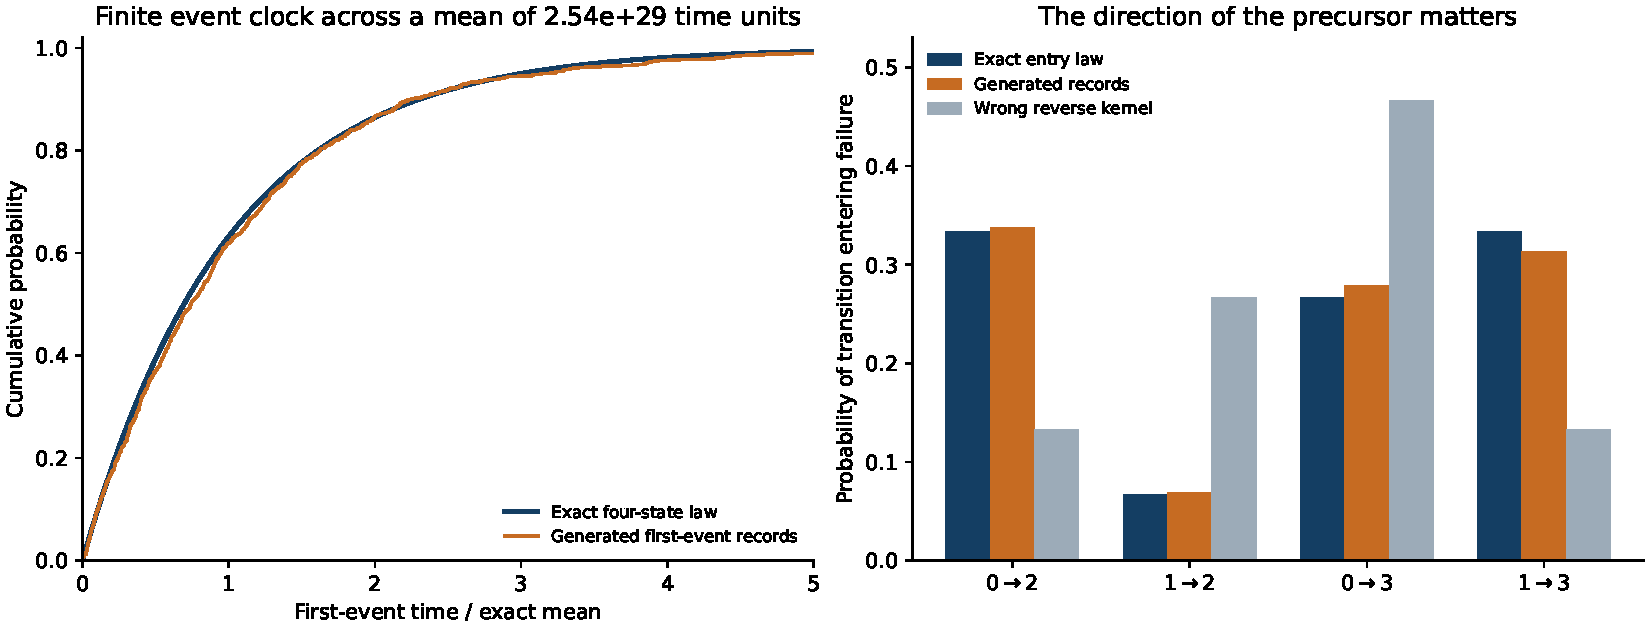
\includegraphics[width=\linewidth]{../next4_execution/event_law_diagnostic.pdf}
\caption{Executed supplied-model diagnostic. Left: generated finite-clock
first-event records against the independent exact law. Right: the entry
transition distribution, including the incorrect boundary reconstruction
that uses the wrong time direction. The small exact solver is a stronger
baseline for this fixture; the plot does not establish practical advantage
for a general exponentially large state space.}
\end{figure}


\section{Preservation and independent destinations}
The preceding 123-file correlated-reliability package is retained byte for byte, including nested passive and deferred calibration packages, all-strength quantum acquisition, the separate global-budget correction, matched parity/GHZ resource law, finite-slew and calibration constructions, thermal effusion with its geometry and exposure bill, reliability curves and their distinct starts, the transport obstruction, passive-memory inequality and useful failed attempts. A before/after hash receipt accompanies the new archive. Originals are unchanged.

Independent constructors owned active model acquisition, exact fixed-law prediction and active thermodynamic identifiability questions before selection. Their full original derivations and source comparisons are retained with their own completion and overlap status. They are not silently made premises of this theorem.

\subsection{Active acquisition and a matching intervention boundary}
The independent active route completes a conditional local-data-to-risk
construction for a known bounded-degree pairwise Gibbs mechanism. Known
neighbor clamps and calibrated compensating fields expose local log odds;
finite holds, readings, field slew and amplitude are priced. The final
construction does not assume that a calibration field preserves an
operating kinetic clock. It prepares a priced focal state and measures the
fast escape separately at every operating context, then uses detailed
balance to reconstruct the slow reverse rate.

An actual finite relaxation-and-safe-rejection preparation yields a
statewise-relative approximation to the equilibrium-safe start. The
earlier changing-law CDF comparison then propagates local factor/rate
confidence and the preparation distortion. The setup requires a repairable
continuing process, all declared variables, faithful clamps/copies,
calibrated fields and positive local relaxation bounds. It does not certify
that a real irreversible catastrophe can be survived during setup.

The matching information bound has exposure proportional to
$e^{(B-H_{\rm field})_+}/(r\eta_{\rm loc}^2)$ when a field cap cannot cancel
a local log-odds barrier $B$, even with adaptive fields and full jump records
under the specified measurement interface. Parameter-independent resets are
granted in that lower bound; field motion is charged in wall time.
The completed source compares active spin-network learning and learning
from Glauber dynamics rather than treating interventions as a new primitive
\cite{jiang,dutt}.

Its four-bit diagnostic used 30,226,360 bit readings and 7,747,360
preparations. The declared single-channel total was
409,497,107.05 model time units. If its rates were per second, this would
be about thirteen years. It is therefore an explicit construction and
resource boundary, not an economical calibration claim. Full proof and
the exact access model are retained in the independent-route source.

\subsection{Exact consistency for a single fixed dynamical law}
The independent mathematical route uses established Lipschitz interpolation
and performance-estimation machinery \cite{ryu}, with exact physical-dimension
qualifications. For one observed transition $f(0)=-e$, $\norm e=1$, a
fixed $L$-Lipschitz map in dimension at least two has the sharp envelope
\[
\sup_f\langle e,f(f(-e))\rangle=
\begin{cases}
-1+L(1+L)/(1+2L),&0\le L\le1/2,\\
L^2-7/8,&L\ge1/2.
\end{cases}
\]
Exact sum-of-squares identities and attaining maps are supplied. At $L=1$,
the value is $1/8$, while the scalar fixed-law value is $-1/3$ and the
specified stepwise outer relaxation gives $1$. The gap comes from retaining
consistency between future transitions of the same map.

For $L<1$, possible equilibria are exactly the intersection of balls
\[
\bigcap_i B\left(
\frac{b_i-L^2a_i}{1-L^2},
\frac{L\norm{b_i-a_i}}{1-L^2}\right)
\quad\text{for data }f(a_i)=b_i.
\]
This gives an actual-dimension second-order-cone formulation for a linear
equilibrium objective and an explicit geometric tail from finite-horizon
to all-time bounds. Low-dimensional rank constraints can remain
nonconvex, and finite observations do not establish the global Lipschitz
prior. General interpolation and Gram methods are established; historical
novelty of the particular sharp envelope is not established.

\subsection{A fixed-mechanics thermodynamic ambiguity}
The independent physical route found substantial prior Astra overlap with
active-port thermodynamic nonidentifiability. Two-temperature Brownian
gyrators are an established physical setting \cite{filliger}. Its retained increment is a
cleaner realization with fixed reciprocal mechanics, unit mobility, bath
directions, port and relaxation rates; only two reservoir temperatures
change. With $A=\operatorname{diag}(1,3)$,
$c=(1,1)^\top/\sqrt2$, $v=(1,-1)^\top/\sqrt2$, set
\[
\Sigma_s=A^{-1}+svv^\top,\qquad
D_s=(A\Sigma_s+\Sigma_sA)/2,\qquad
dX=(-AX+cu)\,dt+\sqrt{2D_s}\,dW.
\]
For $0\le s<4+2\sqrt5$, native stationary starts and output $Y=c^\top X$
give identical complete records under every well-posed causal force
controller. Both state directions are controllable and observable.
At $s=0$ the system is at equilibrium; at $s=4$ it has positive temperatures
$5\pm2\sqrt5$, heat current $4/\sqrt5$, and entropy production $16/5$,
yet the same accessible mechanical transcript.

The unbounded-entropy limit requires a bath temperature tending to zero
and does not imply unbounded heat power. A trusted reset of the full hidden
covariance or an added thermal port breaks the equivalence, but is extra
physical access. Native stationary initialization and ideal white baths
are explicit premises. This is retained as a stricter physical example,
not promoted as a new broad nonidentifiability discovery.

The governing prior publication is pinned at revision
\texttt{fef3640a8b1dc5475674a006de417f652f3baf3c}:
\href{https://github.com/harjassand/astra-research-knowledge/tree/fef3640a8b1dc5475674a006de417f652f3baf3c/research/returns/2026-11-05-p3-correlated-reliability}{Governing correlated-reliability publication}.
Accepted earlier mathematics is used at its stated scope. This work constructs a new operation rather than revalidating those premises.

\begin{thebibliography}{10}
\small
\bibitem{blanchet} J. Blanchet, \emph{Optimal Sampling of Overflow Paths in Jackson Networks}, Mathematics of Operations Research 38 (2013), 698--719. \url{https://doi.org/10.1287/moor.2013.0586}. Author manuscript: \url{https://web.stanford.edu/~jblanche/papers/RareJackson7.pdf}.
\bibitem{koskela} J. Koskela, D. Spano and P. A. Jenkins, \emph{Inference and rare event simulation for stopped Markov processes via reverse-time sequential Monte Carlo}, Statistics and Computing 28 (2018), 131--144. \url{https://doi.org/10.1007/s11222-017-9722-1}.
\bibitem{ops} D. W. H. Swenson et al., \emph{OpenPathSampling: A Python Framework for Path Sampling Simulations. 1. Basics}, J. Chemical Theory and Computation 15 (2019), 813--836. \url{https://doi.org/10.1021/acs.jctc.8b00626}.
\bibitem{we} B. W. Zhang, D. Jasnow and D. M. Zuckerman, \emph{The weighted ensemble path sampling method is statistically exact for a broad class of stochastic processes and binning procedures}, J. Chemical Physics 132 (2010), 054107. \url{https://doi.org/10.1063/1.3306345}.
\bibitem{botev} Z. I. Botev and P. L'Ecuyer, \emph{Sampling Conditionally on a Rare Event via Generalized Splitting}, INFORMS J. Computing 32 (2020), 986--995. \url{https://doi.org/10.1287/ijoc.2019.0936}.
\bibitem{parrep} D. Aristoff, T. Lelievre and G. Simpson, \emph{The Parallel Replica Method for Simulating Long Trajectories of Markov Chains}, Applied Mathematics Research eXpress (2014), 332--352. \url{https://doi.org/10.1093/amrx/abu005}.
\bibitem{aldous} D. Aldous, \emph{Markov chains with almost exponential hitting times}, Stochastic Processes and their Applications 13 (1982), 305--310. \url{https://doi.org/10.1016/0304-4149(82)90016-3}.
\bibitem{zweimuller} R. Zweimuller, \emph{Hitting Times and Positions in Rare Events}, Annales Henri Lebesgue 5 (2022), 1361--1415. \url{https://doi.org/10.5802/ahl.154}.
\bibitem{sharpe} D. J. Sharpe and D. J. Wales, \emph{Numerical analysis of first-passage processes in finite Markov chains exhibiting metastability}, Physical Review E 104 (2021), 015301. \url{https://doi.org/10.1103/PhysRevE.104.015301}.
\bibitem{jiang} J. Jiang, D. A. Sivak and M. Thomson, \emph{Active Learning of Spin Network Models}, arXiv:1903.10474 (2019). \url{https://arxiv.org/abs/1903.10474}.
\bibitem{dutt} A. Dutt, A. Y. Lokhov, M. Vuffray and S. Misra, \emph{Exponential Reduction in Sample Complexity with Learning of Ising Model Dynamics}, Proceedings of Machine Learning Research 139 (2021), 2914--2925. \url{https://proceedings.mlr.press/v139/dutt21a.html}.
\bibitem{ryu} E. K. Ryu, A. B. Taylor, C. Bergeling and P. Giselsson, \emph{Operator Splitting Performance Estimation: Tight Contraction Factors and Optimal Parameter Selection}, arXiv:1812.00146. \url{https://arxiv.org/abs/1812.00146}.
\bibitem{filliger} R. Filliger and P. Reimann, \emph{Brownian Gyrator: A Minimal Heat Engine on the Nanoscale}, Physical Review Letters 99 (2007), 230602. \url{https://doi.org/10.1103/PhysRevLett.99.230602}.
\end{thebibliography}

\end{document}
